\documentclass{article}

% if you need to pass options to natbib, use, e.g.:
% \PassOptionsToPackage{numbers, compress}{natbib}
% before loading nips_2016
%
% to avoid loading the natbib package, add option nonatbib:
% \usepackage[nonatbib]{nips_2016}

\usepackage[final]{Stat212b-Shariq-Mobin-WriteUp}

% to compile a camera-ready version, add the [final] option, e.g.:
% \usepackage[final]{nips_2016}

\usepackage[utf8]{inputenc} % allow utf-8 input
\usepackage[T1]{fontenc}    % use 8-bit T1 fonts
\usepackage{hyperref}       % hyperlinks
\usepackage{url}            % simple URL typesetting
\usepackage{booktabs}       % professional-quality tables
\usepackage{amsfonts}       % blackboard math symbols
\usepackage{nicefrac}       % compact symbols for 1/2, etc.
\usepackage{microtype}      % microtypography
% SHARK
\usepackage{amsmath}
\usepackage{graphicx}
\usepackage{subfig}

\title{Voice Conversion}

% The \author macro works with any number of authors. There are two
% commands used to separate the names and addresses of multiple
% authors: \And and \AND.
%
% Using \And between authors leaves it to LaTeX to determine where to
% break the lines. Using \AND forces a line break at that point. So,
% if LaTeX puts 3 of 4 authors names on the first line, and the last
% on the second line, try using \AND instead of \And before the third
% author name.

\author{
  Shariq A. Mobin \\
  Redwood Center for Theoretical Neuroscience \\
  UC Berkeley \\
  \texttt{shariq.mobin@gmail.com} \\
  %% Affiliation \\
  %% Address \\
  %% \texttt{email} \\
  \And
  Joan Bruna \\
  Department of Statistics \\
  UC Berkeley \\
  \texttt{joan.bruna@gmail.com}
}

\begin{document}
% \nipsfinalcopy is no longer used

\maketitle

\begin{abstract}
    The human auditory system is able to distinguish the vocal source of thousands of speakers, yet not much is known about what features the auditory system uses to do this. Fourier Transforms are capable of capturing the pitch, or harmonic structure, of the speaker but this alone proves insufficient at identifying speakers uniquely. The remaining structure, often referred to as timbre, is critical to identifying speakers yet little is understood about it. In this paper we use recent advances in neural networks in order to manipulate the voice of one speaker into another by transforming not only the pitch of the speaker, but the timbre. We review generative models built with neural networks as well as architectures for creating neural networks that learn analogies. Our preliminary results converting voices from one speaker to another are encouraging.
\end{abstract}

\section{Introduction}
    When audiologists describe what makes the sound of one person to the next sound different they first refer to the pitches of the speakers and second to the timbre of speakers. While pitch is well described by the harmonic structure little is known about what timbre is. Often the pitches can be identical but the way it sounds is completely different. This can heard when a trumpet and piano play the same note, while they have same pitch, the timbre is what gives rise to the strong disparity in perception.
    One can think about vocal signals as being an entanglement of two factors - what the speaker is saying and who is saying it. The vocal signal is a non-stationary process which causes the disentanglement of these two factors to be very difficult. In this paper we will explore if it possible to hold one of these two factors constant and alternate the other. That is, we will see if it is possible to convert the speaker of a vocal signal while holding the word spoken constant.

\section{Background}
\subsection{Constant Q-Transform}
    In theory, we could train our neural network with the raw audio waveformm as input. However, in the signal processing community some type of frequency analysis of the waveform is often analyzed as this transformation makes explicit the harmonic structure of the signal. Here, we apply a constant-Q filter bank wavelet transformation (CQT)to the audio signal. This transformation has a number of desirable properties, the most important are:
\begin{enumerate}
\item The transformation uses logarithmic scaling in frequency. This is very useful when the sound wafeform spans many octaves as in the case of waveforms from the human vocal system.
\item The CQT transformation has very high temporal resolution and low spectral resolution for high frequencies whereas the converse is true for low frequncies. This is very similar to the transformation the basilar membrane of the cochlea in the human auditory system performs on the sound waveform.
\end{enumerate}

\subsection{Deep Visual Analogy Making}
    Deep Visual Analogy Networks \cite{reed2015deep} are a recent neural network architecture that has been able to achieve incredible results rotating sprites in the image domain. The goal of the network is to make analogies: "A is to B as C is to D". That is, given A, B, and C as input we would like to predict D. An example would be: "groom is to bride as king is to queen". The approach taken by this model is to learn an embedding of the input such that solving these analogies is easy, e.g. linear:
\begin{eqnarray*}
\Phi(D) - \Phi(C) \approx \Phi(B) - \Phi(A)
\end{eqnarray*}
This embedding can be visualized in Figure \ref{embed_linear}. In practice the relationship does not have to be linear, the relationship can further be approximated by more neural network layers, as in the case of our model. A visualization of the network can be seen in Figure \ref{analogy_network}.

\begin{figure}[h]
    \centering
    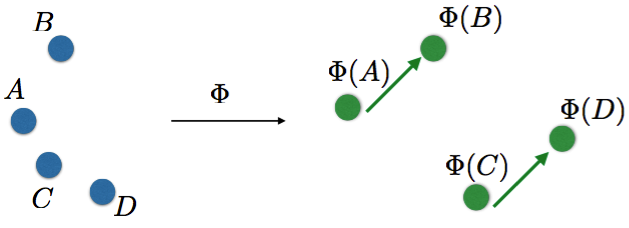
\includegraphics[scale=0.40]{embed_linear.png}
    \caption{By learning an embedding operator, $\Phi$, we are able to linearize the analogy "A is to B as C is to D"}
    \label{embed_linear}
\end{figure}

\begin{figure}[h]
    \centering
    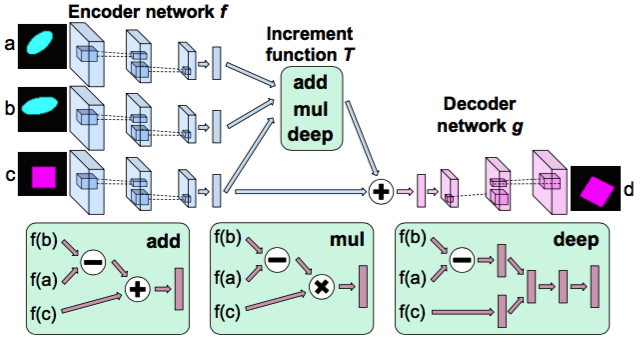
\includegraphics[scale=0.40]{analogy_network.png}
    \caption{A visualization of the Convolutional Neural Network used in the Visual Analogy Network}
    \label{analogy_network}
\end{figure}

Here our objective function is:
\begin{eqnarray*}
E = \sum_{(a,b,c,d)} \frac{1}{2}||d - g(\Phi(b) - \Phi(a) + \Phi(c)||^2
\end{eqnarray*}

\subsection{Generative Adversarial Networks}
Generative adversarial networks (GANs) \cite{goodfellow2014generative} are a recent neural network architecture that allow for very good generative models. These networks have been used in the image domain to create very convincing images of a variety of objects \cite{denton2015deep}. The basic idea is to use one neural network that is a generator and use another neural network as a discriminator. The networks are adversarial in the sense that the generative model is trying to imitate the distribution of some true distribution, e.g. images, while the discriminative network is trying to classify images as coming from the true distribuitoin or the generative, fake, distribution. This is articulated in Figure \ref{adversarial_network}.

\begin{figure}[h]
    \centering
    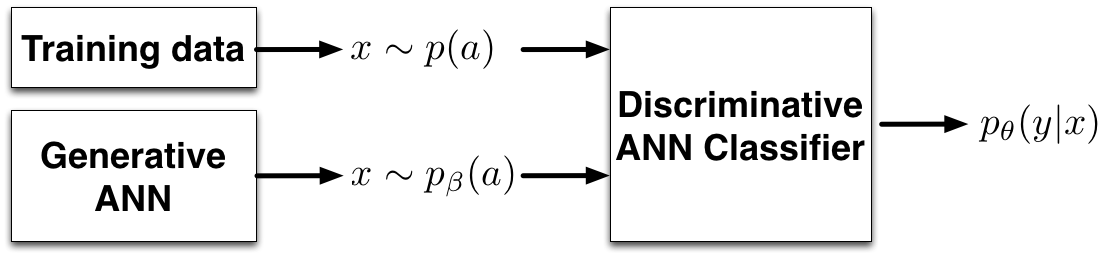
\includegraphics[scale=0.40]{adversarial_network.png}
    \caption{A visualization of the the Generative Adversarial Network idea}
    \label{adversarial_network}
\end{figure}

The goal is then to solve a minimax problem:
\begin{eqnarray*}
\underset{\beta}{\text{min}} \hspace{1mm} \underset{\theta}{\text{max}} \hspace{1mm} \Big[ \mathbb{E}_{x \sim p(a)} \text{log} \hspace{1mm} p_{\theta} (y=\text{`real’}|x) + \mathbb{E}_{x \sim p_{\beta}(a)} \text{log} \hspace{1mm} p_{\theta} (y=\text{`fake’}|x) \Big]
\end{eqnarray*}

In practice optimizing these networks is very difficult and realizes on many tricks.

\section{Model}
Here, we combine the ideas from Deep Visual Analogy Networks (VANs) and Generative Adversarial Networks (GANs) in order to create a model capable of doing voice conversion. A VAN serves as our generative model in the GAN sense. The discriminator of our GAN is then implemented by a classifier which distinguishes not only real and fake CQT samples but what speaker and word category the sample belongs to. This can be summarized by the new minimax equation:

\begin{eqnarray*}
\underset{\beta}{\text{min}} \hspace{1mm} \underset{\theta}{\text{max}} \hspace{1mm} \Bigg[ \sum_{(w,s)} &\mathbb{E}_{x \sim p(a|W=w,S=s)} \text{log} \hspace{1mm} p_{\theta} (W=w, S=s|x) \hspace{1mm} + \\
&\mathbb{E}_{x \sim p_{\beta}(a|W=w,S=s)} \text{log} \hspace{1mm} p_{\theta} (w=\text{`fake'}, s=\text{`fake'}|x) \Bigg]
\end{eqnarray*}

\subsection{Results}

\begin{figure}[h]
    \centering
    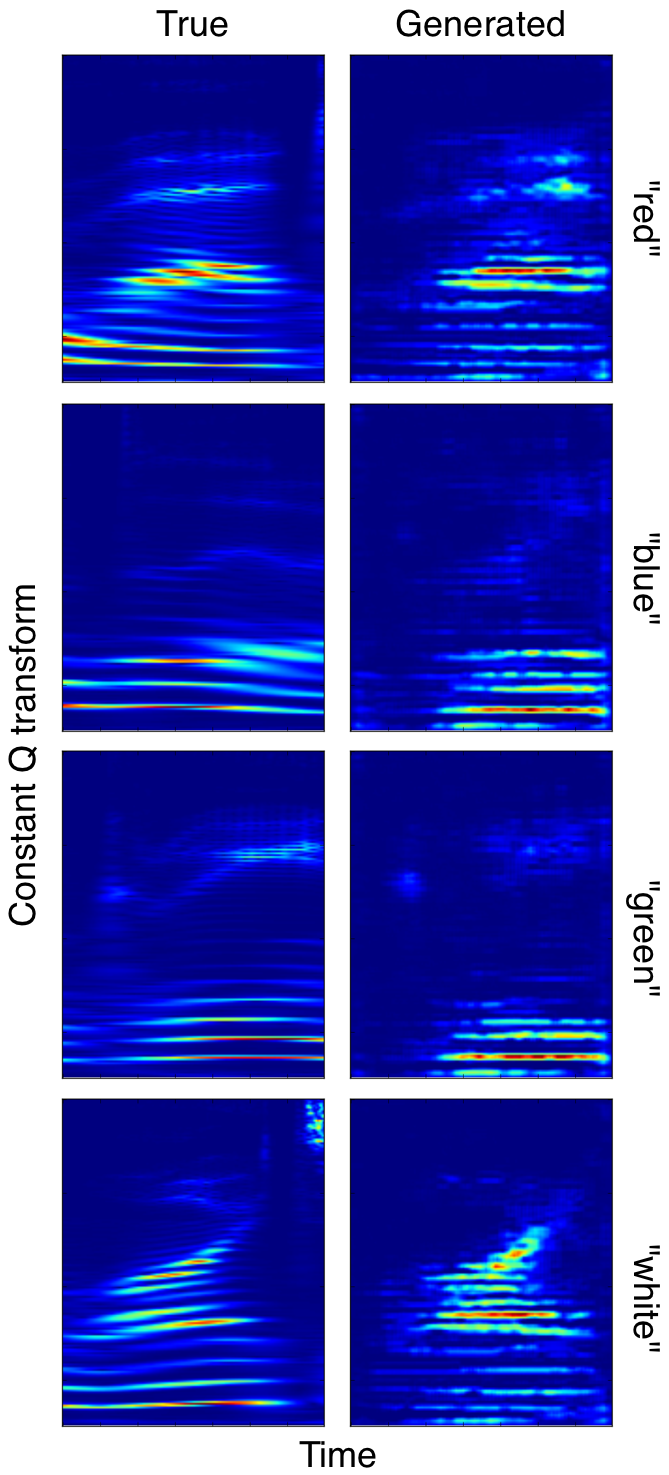
\includegraphics[scale=0.40]{results.png}
    \caption{The left column corresponds to samples of Speaker 2 saying the color indicated on the row from the training data. The right column corresponds to generates samples from our model of the same speaker and color.}
    \label{results}
\end{figure}


\subsection{Conclusion}

{\small
\clearpage
\bibliographystyle{plain}
\bibliography{references.bib}}

\end{document}
